\chapter{Introduction}\label{chap:introduction}

\section{Motivation}\label{sec:motivation}

The amount of information produced and processed in the world has seen a steady increase over the past decades.
The world's internet traffic has been increasing exponentially.
Edholm's Law \cite{Edholm04} predicts that this behaviour should continue until at least 2030.
Edholm's Law is an observation that the total data transmited globally rising in a Moore's Law like pattern\cite{Moore98}: it doubles every $18$ months.

As the amount of data generated by users all around the world increases, the need to store and access this data increases accordingly.
Alongside this evolution there is an expansion on the number of digital services offered to users: musics, videos, books and other types of files and media that can be accessed from anywhere.
So, not only data volume increases but it has to be accessible more reliably than ever 

The solution companies found to provide these services globally is called Cloud Computing, which can be defined as ``a technique where IT services are provided by massive low-cost computing units connected by IP networks''\cite{Qian09}.

However, even though Cloud Computing is sold as a way for users to access computing resources they don't have physical access to, the hardware responsible for this computing power must be placed somewhere.
This is achieved by the establishment of multiple data centers all around the world to which devices from anywhere can connect in order to get access to the desired services.
Microsoft, for example, has 300 data centers worldwide to provide their services to their clients \cite{MicrosoftDataCenters}.

A data center is a complex installation that consists of thousands of hard drives connected by kilometers of optical fiber cables.
Therefore, there are massive amounts of investment done in order to create and maintain these facilities.
Microsoft is investing \$80 billion in order to upgrade their data centers \cite{MicrosoftDataCenters}.
So there is a demand for services related to their maintenance and improvement.

In this context, one of the main aspects of Cloud Computing in general is the strong virtualization and reliability of the system\cite{Qian09}, meaning that even if some of the hardware fails the service should still be provided without interruption.
So, as hardware components fail, they need to be replaced to ensure that the system keeps working for a long time.

Moreover, to maintain a reliable system it is not enough to only replace the hardware after it fails.
In order to prevent some serious issues, such as data loss, without having to permanently have a copy of all the data it is necessary to predict the hardware failures.

Therefore, one of the main problems faced by data centers is the need to detect which pieces of hardware are going to fail before a fatal crash occurs.
The identification of a soon to fail disk makes it possible for it to be replaced beforehand.
This allows both the prevention of data loss and the maintenance of the service reliability.

Out of all the components that are part of a computer, $80\%$ of the failures occur due to the problems on the hard drives, as indicated by Table \ref{devicefailuretable}
Therefore, there is a special focus on predicting failures on disks.

\begin{table}
    \begin{center}
      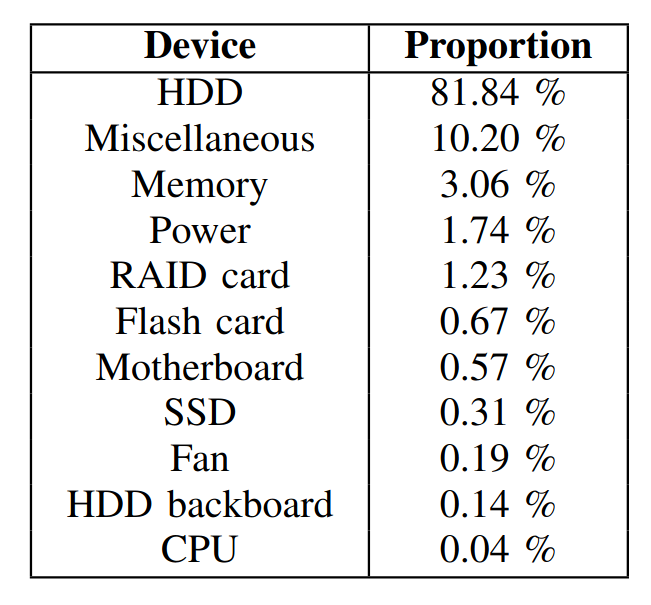
\includegraphics[width=.6\linewidth]{FailureProportions.png}
      \caption[Failure percentage by component]{Data center failure percentage by component - \cite{Wang17}}
      \label{devicefailuretable}
    \end{center}
  \end{table}

Hardware vendors are well aware of this situation and the difficulties related to managing thousands of hard drives.
So, in order to allow their users to better tackle these problems, they added a monitoring system to their drives.
This technology is called SMART (Self-Monitoring, Analysis, and Reporting Technology).

Using this protocol, vendors can provide to users indicators of the disk status to the user.
Some of these attributes are Power-On Hours, Air Flow Temperature and Reallocated Sector Count (number of sectors that had to be copied elsewhere on the disk after a failed read or write operation in order to prevent data loss)\cite{SamsungSSD}.

These disks may also come equipped with a software that is, in theory, able to signal problems with the disk based on the values of the SMART attributes.
However, these systems just compare the SMART values to a threshold that is set by the vendor for each attribute \cite{SamsungSSD}.

Moreover, even when a threshold has been exceeded and a disk is flagged by the software, it does not mean that the disk will suffer an unrecoverable failure.
It often is just a signal that the drive will work more slowly than its specifications indicate.

In addition to that, these status provided by the vendors consider each attribute independently.
They do not take into account the fact that some problems in the hard drive can cause different indicators to increase simultaneously

As a consequence, considering the relationship between different attributes would allow problems to be more accurately detected.
For example, having a huge number of Power-On cycles when compared to Power-On hours may indicate a problem in the disk that causes it to crash and restart constantly.

Finally, this ad-hoc approach uses static values and do not consider the evolution of the attributes over time.
Imagine the situation of a disk that has not reallocated any sectors so far, and at some point the rate at which sectors have to be reallocated increases abruptly.
By taking into account how this attribute evolves over time, this problem can be more quickly detected before the threshold value is reached.

However, even though the built-in failure detection system is not very effective, it doesn't mean that the data itself cannot be used to obtain more interesting results, after all the Hard Drive Failure Prediction Problem must still be solved.
Current research uses mostly machine learning approaches such as SVMs and Neural Networks to tackle this problem.
Further details of how these methods work and how they can be applied to the problem at hand will be detailed in Chapter \ref{chap:background}. 

\section{Problem}\label{sec:problem}

Suppose we have a dataset coming from SMART attribute samples for a certain time period of a data center.
During the observation interval, we also record if each one of the disks has failed in an unrecoverable manner.

The challenge is to train a model able to learn patterns related to the failing disks well enough to be able to identify them before the failure occurs while avoiding to flag the working ones.

Let $x_{i,t}$ be the vector in which the $j^{th}$ component designs the measure of the $j^{th}$ SMART attribute for disk $i$ at time $t$.
For the disks we have observed, we also know a value $y_i$ that is either $0$, if this disk has eventually failed or $1$ if, until the end of the observation period, the disk kept working properly.
Also, let the number of different smart attributes be equal to $m$.

Then given a series of vectors with the SMART attributes for an unseen disk, $\left(\hat{x}_1\dots\hat{x}_t\right)$, we want to output a value $\hat{y}_t$.
Here, $\hat{y}_t$ equal to 0 means that the model predicts that the disk that generated the given sequence is going to fail soon.
A value of $\hat{y}_t$ equal to 1 denotes that there isn't a risk of the hard drive failing in the near future.

In a real world scenario, if the value $\hat{y}_t$ is equal to $0$, then a warning should be sent to the people responsible for maintaining the data center in order to replace the concerned disk.

This corresponds to a more particular classification problem.
Instead of classifying individual samples, we intend to classify sequences as corresponding to working or failing disks.

Therefore, machine learning methods such as Decision Trees and Neural Networks, provide a start point to begin tackling the problem.
However, some additional tools are necessary in order to obtain a verdict for the sequence from the samples that form it.

Here, it is important to describe some particularities of the problem that will allow us to better solve it.
First of all, as we have mentioned, the samples form a time series.
As we will see on Chapter \ref{chap:background}, this can be a motivation to use methods such as Long Short-Term Memory networks (LSTM) that can encode and work with time dependencies.

Moreover, even other methods such as Random Forests that can't easily deal with time dependencies can be extended to make use of the time series aspect of the data.
This is due to the fact that we are able to encode some aspects of the time series and append it to each sample.
More specifically, as we will see in Subsection \ref{subsec:change_rate}, we are able to append information regarding the change rate of our attributes.

A second point that needs to be mentioned is that the amount of disks in each class is not similar at all.
Since a hard drive has a service life of around 3 to 5 years \cite{Vishwanath10}, and observations are performed for a few weeks, no failure will be observed for most of the disks.
The ratio of failing disks over the total amount is between $0.4\%$ and $1.9\%$ \cite{Xu16}.
So, any approach to this problem has to handle this imbalance in the input data.

Thirdly, the meaning of each SMART attribute is not the same for different vendors \cite{SamsungSSD}.
The protocol is standardized, but what it reports is not.
So, an algorithm for failure prediction cannot be trained on data from different vendor disks.
Moreover, in general, it is not a good idea to mix data from different disks on the same dataset, since they can have different failure causes profiles.

Most of the time, the limitation of not being able to mix data about different disk models does not pose a problem to the datasets generated by the data centers.
This is due to the fact that, in practice, a data center uses hundreds of copies of the hardware of the same model and has at most a couple of different models.
This allows for the replacement of failing disks do be done in a cheaper and more swiftly manner, since it simplifies stock management.

The evaluation of the models is done using two main metrics that must be taken into account.
The first one is the FDR (Failure Detection Rate).
This is equal to the ratio between the number of disks that are correctly predicted to be failing and the total amount of failing disks.
Its value should be as close to $1$ as possible.

The second metric is the FAR (False Alarm Rate).
This is equal to the ratio between the number of disks that are wrongly predicted to be failing and the total amount of disks that do not fail.
Its value should be as close to $0$ as possible.

The challenge is to find algorithms that find an equilibrium between this values.
If it predicts every $\hat{x}_t$ to give an output $\hat{y} = 1$, the FAR will be equal to $0$, but the FDR too.
On the other hand, if it predicts every $\hat{x}_t$ to give an output $\hat{y} = 0$, the FDR will be equal to $1$, but the FDR too.
So, we notice that a tradeoff must be done between the FDR and the FAR.

Finding this balance is identical to the Precision-Recall tradeoff problem in most machine learning problems.
This is because, as we are going to show in Section \ref{sec:lstm}, the FDR and the FAR can be mapped to the precision and the recall metrics respectively.

However, both metrics should be treated identically.
Suppose that during a period of one month, $2\%$ of the hard drives in a data center fail.
This corresponds to a lifetime of about 4 years, so it can represent a real world scenario \cite{Vishwanath10}.
If the FDR decreases by $1\%$, then only $0.02\%$ of the disks of the data center will fail without a warning during one month.

In contrast, if the FAR increases by the same amount, then $0.98\%$ of the disks of the whole data center will be unnecessarily replaced during the same period.
This is close to $50\%$ of the disks that actually need to be replaced and can incur a substantial cost.
So, most algorithms in the literature prefer to have a bias towards classifying a disk as working rather than failing.

Aditionnaly, it is impossible to reach perfect values for both indicators.
This is due to the fact that hard drives are subject to real world conditions.
For example, a short circuit on a disk may be caused by an electrical surge, but it does not depend on the internal state of the disk and thus cannot be predicted by any approach using SMART attributes.

There is a third metric we can use to evaluate our models, even though it is usually secondary when compared to the others.
The Time In Advance (TIA) is how much time there was between the moment in which a model warned that a disk was going to fail and the instant it actually did.

The TIA measures how much time, on average, the people responsible for managing a data center have to backup the data from a given disk and replace it to prevent any form of data loss or disruption of service.

The TIA is less important than the FDR and FAR because we don't need to try to maximize it.
It suffices for it to be high enough to allow the team to respond.

In order to prevent the problems mentioned above, oftentimes actions have to be taken considering the worst case scenario.
For the TIA to be high in almost every scenario, it must have a large average while keeping a small standard deviation.

\section{Objectives}

This project has three main objectives.
The first one is to create a library that implement some of the state of the art methods used in research.
The idea is to also made it in such a way that it can be extended with new methods and models in order to allow them to be easily tested and compared to other ones. 

After creating the library, further tests can be performed on existing methods to understand how they evolve as their parameters change.
For example, most work such as \cite{Zhu13} and \cite{Xu16} use different pre and post processing steps and therefore make it harder for them to be objectively compared.
Our intention is to remove any bias that can occur due to these stages.

The third objective is to extend existing methods to also make use of the concept of Health Status introduced by Xu et al.\cite{Xu16}.
The idea is to use the fact that, even though the sequences must be classified in two classes, the samples that form them do not.

So, we increase the number of classes by putting training samples closer to the moment of failure in a different class than the ones that are farther away.
This step will be explained in details on Section \ref{sec:health_status}.

So, the goal is to extend our methods to support more than two classes and study their reaction to this change.
Different models can be extended this way, whether they are other neural network based methods such as \cite{Zhu13} or even if they use other approaches such as the Random Forest one presented by Shen et al.\cite{Shen18}.  